\documentclass[12pt,a4paper,oneside,norsk]{article} 
\usepackage[utf8]{inputenc}
%\usepackage[norsk]{babel}
\usepackage{amsmath}
\usepackage{amsfonts}
\usepackage{amssymb}
\usepackage{makeidx}
\usepackage{graphicx}
\usepackage{hyperref}
\usepackage[left=2cm,right=2cm,top=2cm,bottom=2cm]{geometry}
\usepackage{float}
\usepackage{multirow}
\usepackage{verbatim} %for å kommentere ut ting
\usepackage[nottoc,numbib]{tocbibind}
\usepackage{chngpage} % allows for temporary adjustment of side margins
\usepackage[parfill]{parskip} %for avsnitt
\usepackage[yyyymmdd,hhmmss]{datetime}
\usepackage{comment} 
\usepackage{caption}
\captionsetup[figure]{labelformat=empty}

\raggedbottom

\usepackage{makeidx}
\makeindex

\begin{document}
%her kommer forsiden:
    \begin{titlepage}
    \begin{center}
    \ \\
    \ \\
    \ \\
    \ \\
    \ \\
    \ \\
    The Gentleman's Club \\
    \ \\
    \ \\
    \ \\
    \ \\{\large \bfseries
    The Gentleman's Club Official Alcoholic Beverages Chart\\
    }
    \ \\
    \ \\
    \ \\
    \ \\
    \ \\
    {\large
    Alcoholic Beverages Chart\\
    }
    \ \\
    {\today\ \\}
    \ \\
    \ \\
    \ \\
    \ \\
    \ \\
    \ \\
    \ \\
    \ \\
    \ \\
    \ \\
    \ \\
    \ \\
    \ \\
    \ \\
    \ \\
    \ \\
    \ \\
    \ \\
    \ \\
    \ \\
    \ \\
    \ \\
    \ \\
    \ \\
   	\ \\
    \ \\
    \ \\
    \ \\
   	\ \\
    \ \\
    \end{center}
    \end{titlepage}
    
    \thispagestyle{empty}
\newpage

\setcounter{page}{1}
\pagenumbering{arabic}
%her er innholdsfortegnelsen. Den lages automagisk
\tableofcontents
\newpage

%HER ER EN LITEN BRUKSANVISNING
%Nedenfor er en mal til hvordan man lager en subsubsection
\begin{comment}
%start å klipp og lim herifra, og lim det inn under riktig "subsection":

\subsubsection{Bryggeri: NAVN PÅ ØL}
\paragraph{Kommentar:} SKRIV DIN MENING HER
\newline
-- -- ( SKRIV NAVN OG DATO)

\begin{figure} [H]
\centering
\includegraphics[scale=0.60]{Bilder/Øl/outcomeinterruption.png} %scale justerer størrelsen på bilde. Linjen etterpå er mappen bilde ligger i.
\caption{SKRIV EN BILDE TEKST.}
\end{figure}
\newpage
%stopp med klipp og lim her! --------------------------
\end{comment}


\section{Øl}
\subsection{Bayer}

\subsubsection{Det Lille Bryggeriet: Bjønnøl}
\paragraph{Kommentar:}Kjedelig og smakløst øl. Lever ikke opp til navnet og er ikke verdt pengene.
\newline
-- -- Isak 13.04.2014

\begin{figure} [H]
\centering
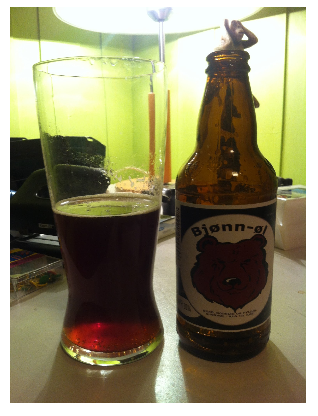
\includegraphics[scale=1.00]{Bilder/Ol/bjonnol.png} %scale justerer størrelsen på bilde. Linjen etterpå er mappen bilde ligger i.
\caption{Bjønnøl fra "Det Lille Bryggeri"}
\end{figure}


\newpage
\subsection{Pils}

\subsubsection{Det Lille Bryggeriet: Birkebeinerpils}
\paragraph{Kommentar:}Nok en skuffende øl fra Det Lille Bryggeriet. Kjedelig og en litt ubehagelig smak i svelget. 
\newline
-- -- Isak 13.04.2014

\begin{figure}
\centering
\includegraphics[scale=0.1]{Bilder/Ol/Birkebeiner.jpg}
\caption{Birkebeinerpils fra Det Lille Bryggeriet}
\end{figure}

\newpage
\section{Vin}

\newpage
\section{Sprit}
\subsection{Whisky}

\newpage
\subsection{Cognac}
\end{document}